\documentclass[a4paper,10pt]{book}
\usepackage[utf8]{inputenc}
\usepackage{physics}
\newcommand*\diff{\mathop{}\!\mathrm{d}}
\usepackage{fullpage}
\usepackage{cite}
\usepackage[utf8]{inputenc}
\usepackage{a4wide}
\usepackage{url}
\usepackage{graphicx}
\usepackage{caption}
\usepackage{float} % para que los gr\'aficos se queden en su lugar con [H]
\usepackage{subcaption}
\usepackage{wrapfig}
\usepackage{color}
\usepackage{amsmath} %para escribir funci\'on partida , matrices
\usepackage{amsthm} %para numerar definciones y teoremas
\usepackage[hidelinks]{hyperref} % para inlcuir links dentro del texto
\usepackage{tabu} 
\usepackage{comment}
\usepackage{amsfonts} % \mathbb{N} -> conjunto de los n\'umeros naturales  
\usepackage{enumerate}
\usepackage{listings}
\usepackage[colorinlistoftodos, textsize=small]{todonotes} % Para poner notas en el medio del texto!! No olvidar hacer. 
\usepackage{framed} % Para encuadrar texto. \begin{framed}
\usepackage{csquotes} % Para citar texto \begin{displayquote}
\usepackage{epigraph} % Epigrafe  \epigraph{texto}{\textit{autor}}
\usepackage{authblk}
\usepackage{titlesec}
\usepackage{varioref}
\usepackage{bm} % \bm{\alpha} bold greek symbol
\usepackage{pdfpages} % \includepdf
\usepackage[makeroom]{cancel} % \cancel{} \bcancel{} etc
\usepackage{wrapfig} % \begin{wrapfigure} Pone figura al lado del texto
\usepackage{mdframed}
\usepackage{algorithm}
%\usepackage{quoting}
\usepackage{mathtools}	
\usepackage{tikz}
\usepackage{paracol}
% tikzlibrary.code.tex
%
% Copyright 2010-2011 by Laura Dietz
% Copyright 2012 by Jaakko Luttinen
%
% This file may be distributed and/or modified
%
% 1. under the LaTeX Project Public License and/or
% 2. under the GNU General Public License.
%
% See the files LICENSE_LPPL and LICENSE_GPL for more details.

% Load other libraries

%\newcommand{\vast}{\bBigg@{2.5}}
% newcommand{\Vast}{\bBigg@{14.5}}
% \usepackage{helvet}
% \renewcommand{\familydefault}{\sfdefault}

\usetikzlibrary{shapes}
\usetikzlibrary{fit}
\usetikzlibrary{chains}
\usetikzlibrary{arrows}

% Latent node
\tikzstyle{latent} = [circle,fill=white,draw=black,inner sep=1pt,
minimum size=20pt, font=\fontsize{10}{10}\selectfont, node distance=1]
% Observed node
\tikzstyle{obs} = [latent,fill=gray!25]
% Invisible node
\tikzstyle{invisible} = [latent,minimum size=0pt,color=white, opacity=0, node distance=0]
% Constant node
\tikzstyle{const} = [rectangle, inner sep=0pt, node distance=0.1]
%state
\tikzstyle{estado} = [latent,minimum size=8pt,node distance=0.4]
%action
\tikzstyle{accion} =[latent,circle,minimum size=5pt,fill=black,node distance=0.4]
\tikzstyle{fijo} =[latent,circle,minimum size=5pt,fill=black]


% Factor node
\tikzstyle{factor} = [rectangle, fill=black,minimum size=10pt, draw=black, inner
sep=0pt, node distance=1]
% Deterministic node
\tikzstyle{det} = [latent, rectangle]

% Plate node
\tikzstyle{plate} = [draw, rectangle, rounded corners, fit=#1]
% Invisible wrapper node
\tikzstyle{wrap} = [inner sep=0pt, fit=#1]
% Gate
\tikzstyle{gate} = [draw, rectangle, dashed, fit=#1]

% Caption node
\tikzstyle{caption} = [font=\footnotesize, node distance=0] %
\tikzstyle{plate caption} = [caption, node distance=0, inner sep=0pt,
below left=5pt and 0pt of #1.south east] %
\tikzstyle{factor caption} = [caption] %
\tikzstyle{every label} += [caption] %

\tikzset{>={triangle 45}}

%\pgfdeclarelayer{b}
%\pgfdeclarelayer{f}
%\pgfsetlayers{b,main,f}

% \factoredge [options] {inputs} {factors} {outputs}
\newcommand{\factoredge}[4][]{ %
  % Connect all nodes #2 to all nodes #4 via all factors #3.
  \foreach \f in {#3} { %
    \foreach \x in {#2} { %
      \path (\x) edge[-,#1] (\f) ; %
      %\draw[-,#1] (\x) edge[-] (\f) ; %
    } ;
    \foreach \y in {#4} { %
      \path (\f) edge[->,#1] (\y) ; %
      %\draw[->,#1] (\f) -- (\y) ; %
    } ;
  } ;
}

% \edge [options] {inputs} {outputs}
\newcommand{\edge}[3][]{ %
  % Connect all nodes #2 to all nodes #3.
  \foreach \x in {#2} { %
    \foreach \y in {#3} { %
      \path (\x) edge [->,#1] (\y) ;%
      %\draw[->,#1] (\x) -- (\y) ;%
    } ;
  } ;
}

% \factor [options] {name} {caption} {inputs} {outputs}
\newcommand{\factor}[5][]{ %
  % Draw the factor node. Use alias to allow empty names.
  \node[factor, label={[name=#2-caption]#3}, name=#2, #1,
  alias=#2-alias] {} ; %
  % Connect all inputs to outputs via this factor
  \factoredge {#4} {#2-alias} {#5} ; %
}

% \plate [options] {name} {fitlist} {caption}
\newcommand{\plate}[4][]{ %
  \node[wrap=#3] (#2-wrap) {}; %
  \node[plate caption=#2-wrap] (#2-caption) {#4}; %
  \node[plate=(#2-wrap)(#2-caption), #1] (#2) {}; %
}

% \gate [options] {name} {fitlist} {inputs}
\newcommand{\gate}[4][]{ %
  \node[gate=#3, name=#2, #1, alias=#2-alias] {}; %
  \foreach \x in {#4} { %
    \draw [-*,thick] (\x) -- (#2-alias); %
  } ;%
}

% \vgate {name} {fitlist-left} {caption-left} {fitlist-right}
% {caption-right} {inputs}
\newcommand{\vgate}[6]{ %
  % Wrap the left and right parts
  \node[wrap=#2] (#1-left) {}; %
  \node[wrap=#4] (#1-right) {}; %
  % Draw the gate
  \node[gate=(#1-left)(#1-right)] (#1) {}; %
  % Add captions
  \node[caption, below left=of #1.north ] (#1-left-caption)
  {#3}; %
  \node[caption, below right=of #1.north ] (#1-right-caption)
  {#5}; %
  % Draw middle separation
  \draw [-, dashed] (#1.north) -- (#1.south); %
  % Draw inputs
  \foreach \x in {#6} { %
    \draw [-*,thick] (\x) -- (#1); %
  } ;%
}

% \hgate {name} {fitlist-top} {caption-top} {fitlist-bottom}
% {caption-bottom} {inputs}
\newcommand{\hgate}[6]{ %
  % Wrap the left and right parts
  \node[wrap=#2] (#1-top) {}; %
  \node[wrap=#4] (#1-bottom) {}; %
  % Draw the gate
  \node[gate=(#1-top)(#1-bottom)] (#1) {}; %
  % Add captions
  \node[caption, above right=of #1.west ] (#1-top-caption)
  {#3}; %
  \node[caption, below right=of #1.west ] (#1-bottom-caption)
  {#5}; %
  % Draw middle separation
  \draw [-, dashed] (#1.west) -- (#1.east); %
  % Draw inputs
  \foreach \x in {#6} { %
    \draw [-*,thick] (\x) -- (#1); %
  } ;%
}



\newcommand{\vm}[1]{\mathbf{#1}}
\newcommand{\N}{\mathcal{N}}
\newcommand{\citel}[1]{\cite{#1}\label{#1}}
\newcommand\hfrac[2]{\genfrac{}{}{0pt}{}{#1}{#2}} %\frac{}{} sin la linea del medio

\newtheorem{midef}{Definition}
\newtheorem{miteo}{Theorem}
\newtheorem{mipropo}{Proposition}

\theoremstyle{definition}
\newtheorem{definition}{Definition}[section]
\newtheorem{theorem}{Theorem}[section]
\newtheorem{proposition}{Proposition}[section]

%http://latexcolor.com/
\definecolor{azul}{rgb}{0.36, 0.54, 0.66}
\definecolor{rojo}{rgb}{0.7, 0.2, 0.116}
\definecolor{rojopiso}{rgb}{0.8, 0.25, 0.17}
\definecolor{verdeingles}{rgb}{0.12, 0.5, 0.17}
\definecolor{ubuntu}{rgb}{0.44, 0.16, 0.39}
\definecolor{debian}{rgb}{0.84, 0.04, 0.33}
\definecolor{dkgreen}{rgb}{0,0.6,0}
\definecolor{gray}{rgb}{0.5,0.5,0.5}
\definecolor{mauve}{rgb}{0.58,0,0.82}

\newif\ifen
\newif\ifes
\newcommand{\en}[1]{\ifen#1\fi}
\newcommand{\es}[1]{\ifes#1\fi}
\estrue


%opening
\title{\huge Algoritmos para la inferencia de habilidad y el aprendizaje social}
\author{Gustavo Landfried}


\begin{document}

\maketitle

\tableofcontents

\chapter{Sistemas naturales de procesamiento de información}

En el último tercio de la historia del Universo, en algún momento hace aproximadamente 4500 millones de años, apareció en la tierra una forma de organización de la materia capaz de auto-replicarse.
El crecimiento de estos linajes son procesos multiplicativos y ruidoso: secuencias de probabilidades de supervivencia y reproducción.
Los errores producidos durante la replicación diversificaron las formas de vida, y las tasas de crecimiento de las diferentes estrategias favorecieron a aquellas mejor adaptadas al ambiente.
Desde aquel momento hasta entonces la vida adquirió una extraordinaria complejidad.
%
\begin{figure}[H]
    \centering
    \begin{subfigure}[b]{0.65\textwidth}
    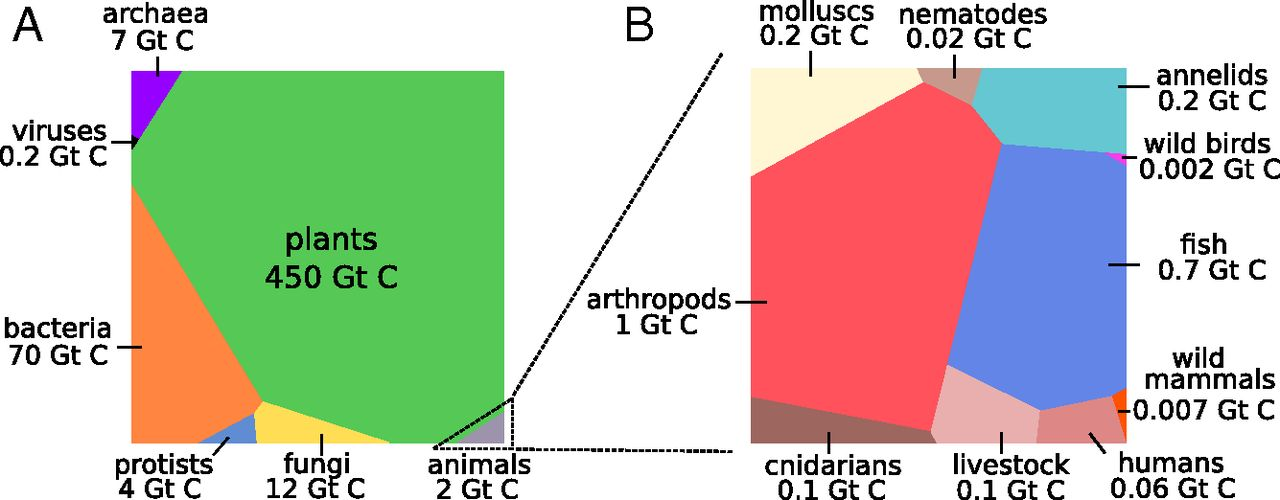
\includegraphics[width=\linewidth]{static/biomass.jpg}
    \end{subfigure}
    \caption{
	Estimación de la distribución actual de la biomasa en la tierra realizada por Bar-On~\cite{barOn2018-biomass}.
    }
    \label{fig:cpr_individual}
\end{figure}
%
Esta complejidad es consecuencia de una serie de transiciones evolutivas~\cite{maynardSmith1995-majorTransitions} en las que las entidades capaces de replicarse de forma independiente, cediendo algo de valor a las otras, pasan a formar unidades evolutivas de nivel superior.
Algunos ejemplos paradigmáticos son la transición de las moléculas replicantes a las protocélulas, la endosimbiosis de las mitocondrias y los plastos por parte de las células eucariotas, la aparición de los organismos multicelulares.
¿Cómo se explica esta tendencia permanente de la vida en favor de la agregación cooperativa?

\section{Evolución}

En evolución, el crecimiento de los linajes en el tiempo, $\omega(t)$, esta gobernado por una secuencias estocástica de tasas de supervivencia y reproducción $f(\cdot)$ dependientes de un ambiente aleatorio $a$,
%
\begin{equation} \label{eq:modelo_exponencial}
\omega_e(T) = \prod_t^T f_e(a(t))
\end{equation}
%
donde $a(t)$ representa el estado del ambiente en el tiempo $t$.
Supongamos que la naturaleza lanza una moneda,
\begin{equation} \label{eq:estrategia_base}
f_e(a) =
\begin{cases}
 1.5 & a = \text{ Cara } \\
 0.6 & a = \text{ Seca }
\end{cases}
\end{equation}
Si sale cara la población se reproduce un 50\% y si sale seca sobrevive el 60\%.

% Parrafo

Según el modelo estándar de evolución, conocido como \emph{replicator dynamic} \cite{taylor1978-replicatorDynamic, schuster1983-replicatorDynamics, hofbauer2003-evolutionaryGameDynamics}, el cambio de la proporción de una estrategia $e$ en la población, $x_e$, está determinado por su tasa de crecimiento caracterísitica $f_e$,
\begin{equation} \label{eq:replicator_dynamic}
x_e^\prime = \frac{x_e f_e}{X}
\end{equation}
donde $X=\sum_i x_i f_i$ es una constante de normalización.
¿Pero cuál es la tasa de crecimiento característica, $f_e$?

% Parrafo

La estimación de la tasa de crecimiento característica, $f_e$, requiere considerar explícitamente la variablidad del ambiente, $a$, y el tipo de proceso que genera esa variabilidad.
Buena parte de la literatura en evolución considera que la estimación correcta se obtiene mediante el valor esperado de los recursos en el tiempo, $\omega(t)$.
Sea $\Omega_t$ el valor de todos los posibles trayectorias en el tiempo $t$, el valor esperado se obtiene pesando cada estado $\omega \in \Omega_t$ por la probabilidad de que ocurran $P(\omega)$
\begin{equation}
\langle \omega \rangle_t = \sum_{\omega \in \Omega_t} \omega \cdot  P(\omega)
\end{equation}

% Parrafo

El valor esperado de la estrategia considerada en la ecuación \ref{eq:estrategia_base} es en los dos primeros pasos temporales de, 
\begin{equation}
\begin{split}
\langle \omega \rangle_1 & = 1.5 \cdot \frac{1}{2} + 0.6 \cdot  \frac{1}{2} = 1.05 \\ 
\langle \omega \rangle_2 &=  1.5^2 \cdot \frac{1}{4} + 2 (0.6 \cdot 1.5 \cdot \frac{1}{4} ) + 0.6^2 \cdot \frac{1}{4}= 1.05^2
\end{split}
\end{equation}
Según el valor esperado, la tasa de crecimiento estimada es $5\%$ por cada paso temporal, $\langle \omega \rangle_t = 1.05^t$.
Y efectivamente eso es lo que ocurre con el promedio de una muestra suficientemente grande de trayectoria individuales en el tiempo, $\omega(t)$, 

\begin{figure}[H]
    \centering
    \begin{subfigure}[b]{0.45\textwidth}
    \includegraphics[width=\linewidth]{figures/pdf/ergodicity_expectedValue.pdf}
    \end{subfigure}
    \caption{
    Promedio de los recursos individuales en el tiempo para diferentes tamaños de la población, en escala logarítimica ($10^0,10^1,10^2,10^3,10^4$).
    A medida que aumentamos el tamaño de la población, el promedio se acerca al valor esperado $\langle \omega \rangle_t = 1.05^t$.
    }
    \label{fig:ergodicity_expectedValue}
\end{figure}

Sin embargo, el valor esperado no representa lo que lo le ocurre a los agentes en el tiempo. 
Individualmente, todas las trayectorias pierden a largo plazo a una tasa cercana al 5\%.
\begin{figure}[H]
    \centering
    \begin{subfigure}[b]{0.45\textwidth}
    \includegraphics[width=\linewidth]{figures/pdf/ergodicity_individual_trayectories.pdf}
    \caption{}
    \label{fig:ergodicity_individual_trayectories}
    \end{subfigure}
    \begin{subfigure}[b]{0.45\textwidth}
    \includegraphics[width=\linewidth]{figures/pdf/ergodicity_individual_trayectories_longrun.pdf}
    \caption{}
    \label{fig:ergodicity_individual_trayectories_longrun}
    \end{subfigure}
    \caption{
    La recta negra representan el valor esperado.
    Figura \ref{fig:ergodicity_individual_trayectories}: tamaño de los recursos individuales en el tiempo, $ \log(\omega(t))$.
    Figura \ref{fig:ergodicity_individual_trayectories_longrun}: con suficiente tiempo todas las trayectorias individuales pegan a la recta azul. 
    }
    \label{fig:cpr_individual}
\end{figure}

La diferencia entre el valor esperado y lo que le ocurre a los agentes individuales en el tiempo es un problema bien conocido en mecánica estadística, llamado ``no-ergodicidad''~\cite{peters2019-ergodicityEconomics}.
Cuando un proceso es ergódico, las descripciones de su dinámica pueden remplazarse mediante el valor esperado, eliminado el tiempo de los modelos.
Sin embargo, las condiciones de para que un sistema cumpla con la hipótesis de ergodicidad son muy restrictivas.
Cuando las hipótesis no se cumplen nos vemos obligados a analizar directamente su dinámica. 

La dinámica evolutiva está gobernada por un procesos multiplicativos (eq.~\ref{eq:modelo_exponencial}), que en un cierto tiempo $t$ puede expresarse como,
\begin{equation}
\omega(T) = \prod^T_{t} f(a(t)) = f(\text{cara})^{n_1} f(\text{seca})^{n_2}
\end{equation}

donde $n_1$ y $n_2$ representa la cantidad de ocurrencias de $f(\text{cara})$ y $f(\text{seca})$, con $n_1 + n_2 = T$.
Las trayectorias observadas en la figura \ref{fig:ergodicity_individual_trayectories} son variables, pero cuanto más tiempo observemos el sistema más suave se vuelven esas líneas (figura \ref{fig:ergodicity_individual_trayectories_longrun}).
En el límite, $T \rightarrow \infty$ todas las trayectoria individuales estarán determinadas por el mismo factor efectivo $\overline{f}$ por el que se multiplica los recursos $\omega(T)$ en cada iteración.
\begin{equation}
\begin{split}
\lim_{T \rightarrow \infty} \omega(T) & = \overline{f}^T \\
\left( \lim_{T \rightarrow \infty} \omega(T) \right)^{1/T} & =  \overline{f} \\
\lim_{T \rightarrow \infty} f(\text{cara})^{n_1/T} f(\text{seca})^{n_2/T} & 
 \end{split}
\end{equation}
Donde las frecuencias $\frac{n_1}{T}$ y $\frac{n_2}{T}$ en el límite $T \rightarrow \infty$ son iguales a las probabilidades de ocurrencia de los estados del sistema.
Por lo tanto, la mejor estimación de la tasa de crecimiento es,
\begin{equation}
\overline{f} = (1.5 \cdot 0.6)^{1/2} \approx 0.95
\end{equation}


Esta fórmula, que permite computar la tasa de crecimiento caracterísitica a largo plazo de las trayectorias individuales, se la conoce también como \emph{media geométrica} y ha sido usada previamente en la literatura de evolución~\cite{dempster1955-geometricMean}.
Una propiedad importante es que su valor siempre es menor que el promedio de estados.
Esto se debe a que en los procesos multiplicativos los impactos físicos de las pérdidas suelen ser más fuertes que los de las ganancias.
En el extremo, un único cero en la productoria alcanza para generar su extinción.

% Decimos que un proceso es ergódico si se cumple que,
% \begin{equation}
%  \underbrace{\lim_{T \mapsto \infty} \frac{1}{T} \sum_{t=1}^T \omega(t)}_{\text{Media temporal}}  = \underbrace{\sum_{\omega} \omega \cdot p(\omega)}_{\text{Media de estados}}
% \end{equation}
% 

\subsection{Ventaja de la cooperación}

En los procesos no-ergódicos, las fluctuaciones tienen un efecto negativo en la tasa de crecimiento individual a largo plazo, pero no en la tasa de crecimiento del valor esperado.
Dado que la varianza realmente importa, una forma eficaz de reducirla es compartir los riesgos~\cite{yaari2010-cooperationEvolution, peters2015-evolutionaryAdvantageOfCooperation}.
%Parafraseando a Den Boer~\cite{denBoer1968-spreadingRisk}, la  supervivencia de una población depende de la distribución del riesgo dentro de la población y entre las poblaciones de diferentes especies.
Ole Peters~\cite{peters2015-evolutionaryAdvantageOfCooperation} considera las consecuencias que la distribución del riesgo de una estrategia cooperativa sencilla tiene sobre la tasa de crecimiento de los agentes.

Los agentes cooperadores simplemente reparten sus recursos en partes iguales luego de cada iteración.

\begin{figure}[H]
\centering
\scalebox{0.75}{
\tikz{

    \node[latent, minimum size=2cm ] (x1_0) {$\omega_1(t)$} ;
    \node[latent, below=of x1_0, minimum size=2cm ] (x2_0) {$\omega_2(t)$} ;

    \node[latent, right=of x1_0, minimum size=3cm ] (x1_0g) {$ \omega_1(t)\cdot f(r_1(t))$} ;
    \node[latent, right=of x2_0, minimum size=1.8cm, xshift=0.6cm , align=left] (x2_0g) {$\omega_2(t)\cdot$\\$f(r_2(t))$} ;
    
    \node[latent, right=of x1_0g, minimum size=3.8cm, yshift=-1.33cm, align=right] (x_0) {$\omega_1(t)\cdot f(r_1(t))$\\$+\omega_2(t)\cdot f(r_2(t))$ } ;
    
    \node[const, above=of x_0] (nx_0) {$\overbrace{\text{Pool}\hspace{2.5cm}\text{Share}}^{\text{\normalsize Cooperaci\'on}}$} ;
    
    \node[latent, right=of x1_0g, minimum size=2.5cm,  xshift=4.5cm] (x1_1) {$\omega_1(t+1)$ } ;
    \node[latent, below=of x1_1, minimum size=2.5cm, yshift=0.7cm] (x2_1) {$\omega_2(t+1)$ } ;
    
    \edge {x1_0} {x1_0g};
    \edge {x2_0} {x2_0g};
    \edge {x1_0g,x2_0g} {x_0};
    \edge {x_0} {x1_1,x2_1};
    
}
}
\caption{Estrategia cooperativa. Los agentes comienzan con los mismos recursos iniciales. Luego crecen independientemente de acuerdo con la ecuaci\'on \ref{}. Luego cooperan poniendo sus recursos en un fondo común, que finalmente es dividio en partes iguales.}
\label{fig:protocolo}
\end{figure}

Las poblaciones enteramente cooperadoras reducen sus fluctuaciones, lo que genera una aumento en la tasa de crecimiento de todos sus miembros.
En la figura \ref{fig:cpr_absolute_cooperation} mostramos la trayectoria de uno de los agentes cooperadores.

\begin{figure}[H]
    \centering
    \begin{subfigure}[b]{0.45\textwidth}
    \includegraphics[width=\linewidth]{figures/cpr_absolute_cooperation.pdf}
    \end{subfigure}
    \caption{
    Tamaño logarítimico de los recursos de un individuo de una población con 33 agentes que comparten su riqueza luego de cada iteración.
    La recta negra que baja representa el promedio temporal, y la que sube el promedio de estados.
    }
    \label{fig:cpr_absolute_cooperation}
\end{figure}

Mediante la cooperación, las poblaciones de agentes logran acceder a tasas de crecimiento individuales equivalentes al promedio de estados del sistema, que en los sistemas no-ergódicos es siempre superior que el promedio temporal.

% Parrafo

Ole Peters considera que este aumento de la tasa de crecimiento demuestra la ventaja evolutiva de la cooperación, lo que propone como principal explicación de las transiciones evolutivas.
Sin embargo Ole Peters no analiza el problema de la deserción, quien dice ``our cooperators are unable to break the cooperative pact''.
No parece ser un problema menor, teniendo en cuenta la tentación que podría significar dejar de aportar al fondo común mientras se siguen recibiendo los beneficios de este.

\subsection{Transiciones evolutivas}

\todo[inline]{subsección no terminada}

Para discutir este punto en detalle, analizamos las tasas de crecimiento de las estrategias cooperadora y desertora en un caso concreto.


\begin{figure}[H]
    \centering
    \begin{subfigure}[b]{0.45\textwidth}
    \includegraphics[width=\linewidth]{figures/cpr_absolute_cooperation_defection_costo.png}
    \end{subfigure}
    \caption{
    Población de 100 agentes, a) totalmente cooperadores, b) con un desertor, c) con 10 desertores.
    }
    \label{fig:cpr_absolute_cooperation_defection_costo}
\end{figure}

Las estrategias desertoras, al evitar compartir sus recursos generan un aumento en sus propias fluctuaciones, afectando su tasa de crecimiento a largo plazo sin necesidad de introducir castigos.
Esto parecería apoyar la idea de Ole Peters de que la cooperación no es altruista sino que está impulsada por el interés personal.
Sin embargo, los agentes evolutivos no son agentes económicos, su frecuencia cambia en base a tasa de \emph{diferencial} de crecimiento.
Por más que la mutua cooperación sea mejor en términos absolutos, un mutante desertor tendrá una tasa de crecimiento mayor a la de su comañero cooperador, por lo que invadirá evolutivamente la población. 

\section{La transición cultural}

La especial integraci\'on de los procesos biol\'ogicos, cognitivos y sociales que permiten a los humanos desarrollar culturas complejas se debió a una coevolución genético-cultural que se desencadenó por el desarrollo previo de la crianza cooperativa~\cite{hrdy2020-emotionallyModern}.
Antes del surgimiento de los humanos \emph{anatómicamente} modernos (masa cerebral actual) y de los humanos \emph{conductualmente} modernos (lenguaje), surgió en África una linaje \emph{emocionalmente} moderno~\cite{hrdy2020-emotionallyModern}.
La forma en la que estos homininos organizaron la crianza produjo un ambiente que favoreció la selección de jóvenes capaces de monitorear y comprender las intenciones de los demás, y de atraer la atención de sus cuidadadores de modo de compartir sus propias necesidades.

% Parrafo

La empatía fue la que permitió el desarrollo del Homo sapiens: la comprensión mutua, la imitación, el lenguaje y finalmente la cultura.
Esta costosa habilidad cognitiva es especialmente eficiente para la adquisición de tradiciones complejas.
Lo que antes debía ser redescubierto una y otra vez mediante costosa experiencia individual, ahora podía ser transmitido a la siguiente generación.
La capacidad de adquirir comportamientos basados en la experiencia de otros sin tener que re-construirlos cada vez por prueba y error conduce un proceso de evolución y acumulativa cultural que permite a las poblaciones humanas adaptarse rápidamente ante cambios bruscos en el ambiente o migraciones a nuevos entornos.

% Parrafo

El surgimiento de la cultura produjo cambios radicales para nuestra especie.
Antes de la transición cultural, estuvimos en grave peligro de extinción, lo que se evidencia en la baja diversidad del genoma humano.
Luego de la transición cultural, en pocos años nuestra especie ocupó todos los nichos ecológicos de la tierra como ningún otro vertebrado terrestre lo había logrado antes.
Esta proeza se logró mediante los sistemas culturales y tecnológico desarrollados por sociedades cazadores-recolectores.
Caminando salimos de África, ocupamos Asia, y de allí Oceanía y las Américas (las flechas del mapa~\ref{fig:agricultura}).
La información transgeneracional fue la que le permitió a estas sociedades simples adaptarse rápidamente a los nuevos desafíos ecológicos.

% Parrafo

El cambio climático ocurrido al inicio del Holoceno (hace 12000 años) propició el desarrollo de la agricultura, que surgió de manera independiente en los seis grandes sistemas geográficos de la tierra: en la región central de África subsahariana, en Asia occidental, en Asia oriental, en Oceanía norte, en América del norte y en América del sur (las puntos rojos del mapa~\ref{fig:agricultura}).
\begin{figure}[H]
    \centering
    \begin{subfigure}[b]{0.6\textwidth}
     \includegraphics[width=\textwidth]{figures/agricultura.pdf}
     \label{fig:agricultura}
    \end{subfigure}
%     \begin{subfigure}[b]{0.40\textwidth}
%     \includegraphics[width=\textwidth]{static/polynesia.png} 
%     \caption{Poblamiento del océano Pacífico}
%     \label{fig:polynesia}
%     \end{subfigure}
    \caption{
    Proyección políedrica de la tierra que conserva los tamaños relativos de los continentes.
    Las felchas indican el poblamiento, desde África a Asia, y de Asia hacia Oceanía y América.
    Los puntos rojos indican surgimiento independiente de agricultura.
    }%
    \label{fig:poblamiento}
\end{figure}
%
Alrededor de estos puntos se desarrollaron los principales centros poblacionales de la humanidad.
El aumento de la población promovió, a su vez, el desarrollo de nuevas innovaciones tecnológicas y científicas, como la escritura, la matem\'aticas, las ingenier\'ias, la astronomía, las ciencias políticas, entre otras.
Durante el año 1400 el mundo florecía de sociedades "prósperas"~\cite{dussel2004-sistemaMundo}: Aztecas en Ámerica del norte, Incas en Ámerica del sur, Tongas en el Pacífico, Bantúes en África sub-sahariana, los Árabes e Indios en Asia occidental y Chinos en Asia oriental, por mencionar algunos.

\subsection{Evolución cultural}

La especie humana posee la peculiar capacidad de desarrollar innovaciones culturales a lo largo de m\'ultiples generaciones, un fen\'omeno denominado \emph{evoluci\'on cultural acumulada}~\cite{Derex2020} (o \textbf{CCE} por sus siglas en ingl\'es).
El modelo causal b\'asico de la literatura de evoluci\'on cultural afirma que la adaptaci\'on humana depende, adem\'as de la experiencia individual y los cambios en el ambiente, de la informaci\'on cultural a la que tienen acceso los agentes.

\begin{figure}[H]
	\centering
	\tikz{
    	\node[accion] (a) {} ;
	    \node[const,below=of a] (na) {Adaptaci\'on} ;
	    \node[accion,above=of a, xshift=-0.8cm] (e) {} ;
	    \node[const,left=of e] (ne) {Experiencia} ;
	    \node[accion,above=of a, xshift=0.8cm] (s) {} ;
	    \node[const,right=of s] (ns) {Informaci\'on cultural} ;
	    \node[accion,above=of a, yshift=0.6 cm] (m) {} ;
	    \node[const,above=of m] (nm) {Medio ambiente} ;
	    \edge {e,s,m} {a};
	}
	\caption{Representaci\'on gr\'afica de un modelo causal para la adaptaci\'on humana.}
\end{figure}

Todas las tecnolog\'ias surgen como resultado de esfuerzo transgeneracionales.
Basada en los principios b\'asicos de la teor\'ia evolutiva (descendencia, modificaci\'on y selecci\'on), la antropolog\'ia ha desarrollado un marco te\'orico para explicar c\'omo cambia la cultura en el tiempo.
Este marco ha motivado el desarrollo de los primeros modelos matem\'aticos para explicar distintas din\'amicas poblacionales de producci\'on, transmisi\'on y mantenimiento de informaci\'on cultural~\cite{cavalliSforza1981-culturalTransmission,boyd1985-evolutionaryProcess}.

% Parrafo

Una idea central en estos trabajos es que el aprendizaje social (por imitaci\'on, observaci\'on, etc.) no es al azar, sino que los individuos eligen de qui\'en aprender.
Por ejemplo, una estrategia simple consiste en copiar lo que hace la mayor\'ia (\emph{frequency-based strategy}).
Otra estrategia t\'ipica toma como modelo de referencia a las personas m\'as exitosas o prestigiosas (\emph{payoff-based strategy}). %, y llama a los individuos exitosos (de los cuales otros individuos aprenden) \textbf{demostradores}.
Las diferentes estrategias de aprendizaje social que se han propuesto~\cite{rendell2010-socialLearningTournament} pueden ser clasificadas entre aquellas que identifican de qui\'enes aprenden los individuos, y aquellas que especifican las circunstancias bajo las cuales los individuos copian a otros.
Por ejemplo, mantener compa\~neros de equipo estable est\'a relacionado con un mayor aprendizaje~\cite{Landfried2019}.

\todo[inline]{Subsección no terminada}

% Parrafo

\section{Objetivos}

\todo[inline]{Sección objetivos}

\chapter{Conocimiento empírico}

\epigraph{El conocimiento empírico no es más que principio de incertidumbre compatible con la evidencia formal y empírica}{}

La ciencia es una institución humana que tiene pretención de verdad.
Las ciencias formales validan sus proposiciones mediante teoremas, resultados derivados de aplicar las reglas internas a un sistema axiomático cerrado.
Las ciencias empíricas, por el contrario, deben validar sus proposiciones dentro de sistemas abiertos, lo que impone siempre un grado de incertidumbre asociada.
¿Cuál es entonces la fuente de validez del conocimiento empírico?

\subsection{Principio de incertidumbre}

Supongamos que tenemos tres cajas y sabemos que detrás de una hay un regalo.
Al no tener certeza de su posición, nos vemos ante la obligación de repartir nuestra creencia entre las posibles opciones.
A las diferentes formas de dividir la creencia le vamos a llamar \emph{distribución de creencias}.
Una posible distirbución de creencias es,

\begin{figure}[H]
\centering
\tikz{ %
        
         \node[factor, minimum size=1cm] (p1) {} ;
         \node[factor, minimum size=1cm, xshift=1.5cm] (p2) {} ;
         \node[factor, minimum size=1cm, xshift=3cm] (p3) {} ;
         \node[const, above=of p1, yshift=.15cm] (fp1) {$1/10$};
         \node[const, above=of p2, yshift=.15cm] (fp2) {$8/10$};
         \node[const, above=of p3, yshift=.15cm] (fp3) {$1/10$};
        } 
\end{figure}

lo que representa una preferencia parcial por la caja del medio.
Pero si de verdad no tenemos ninguna información respecto de dónde está el regalo, no hay motivos para tener preferencia por ninguna de las opciones, lo que sin lugar a dudas nos hará estar de acuerdo en la necesidad de dividir la creencia en partes iguales.
Éste es un viejo principio conocido como ``de indiferencia''.

\begin{figure}[H]
\centering
\tikz{ %
        
         \node[factor, minimum size=1cm] (p1) {} ;
         \node[factor, minimum size=1cm, xshift=1.5cm] (p2) {} ;
         \node[factor, minimum size=1cm, xshift=3cm] (p3) {} ;
         \node[const, above=of p1, yshift=.15cm] (fp1) {$1/3$};
         \node[const, above=of p2, yshift=.15cm] (fp2) {$1/3$};
         \node[const, above=of p3, yshift=.15cm] (fp3) {$1/3$};
        } 
\end{figure}

Este tipo de distribuciones de creencias, que permiten el acuerdo intersubjetivo, la vamos a llamar \textbf{creencia honesta}.
Elegimos el término ``intersubjetividad'', por sobre el de ``subjetividad'', debido a que el primero connota el cumplimiento de las condiciones que producen al acuerdo entre las conciencias individuales, mientras que el segundo connota una arbitrariedad que lo obstaculiza.
Elegimos el término ``intersubjetividad'', por sobre el de ``objetividad'', porque el primero connota una actividad construcitva entre los sujetos, mientras que el segundo connota la imposición directa del objeto sobre los sujetos.

% Parrafo

%Una propiedad común a todas las creencias honestas es la maximización de la incertidumbre (manteniendo la coherencia con la información disponible).
%La distribución con menor incertidumbre es la que asigna toda la creencia a una de las opciones.
%La distirbución más lejana a esta, 
%En este caso, en el que no tenemos información previa, la obtuvimos dividiendo la creencia en partes iguales.
Tenemos entonces un principio para alcanzar acuerdos en los casos en los que no tenemos información previa.
¿Pero cómo hacemos para alcanzar acuerdos cuando recibimos nueva información?

\section{Evidencia formal y empirica}

Supongamos que recibimos el dato de que el regalo no está en la caja del medio, lo que nos permite asignar creencia 0 a esa caja.

\begin{figure}[H]
\centering
\tikz{ %
         \node[factor, minimum size=1cm] (p1) {} ;
         \node[det, minimum size=1cm, xshift=1.5cm] (p2) {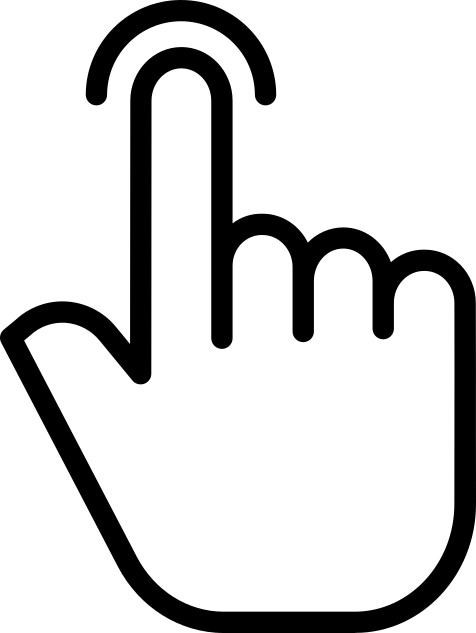
\includegraphics[width=0.03\textwidth]{static/dedo.png}} ;
         \node[factor, minimum size=1cm, xshift=3cm] (p3) {} ;

         \node[const, above=of p1, yshift=.15cm] (fp1) {$?$};
         \node[const, above=of p2, yshift=.15cm] (fp2) {$0$};
         \node[const, above=of p3, yshift=.15cm] (fp3) {$?$};
         \node[const, below=of p2, yshift=-.10cm, xshift=0.3cm] (dedo) {};
        } 
\end{figure}

Para actualizar el resto de las cajas necesitamos interpretar qué nos está diciendo la pista.
Supongamos que la pista depende de dónde está el regalo, sólo nos puede indicar dónde no está el regalo.
Esto lo podemos representar con el siguiente modelo causal.

\begin{figure}[H]
\centering
\tikz{            
    \node[latent,] (r) {
\includegraphics[width=0.06\textwidth]{static/regalo.png}} ;
    \node[const,left=of r] (nr) {\Large $r$} ;    
    
    
    \node[latent, below=of r] (d) {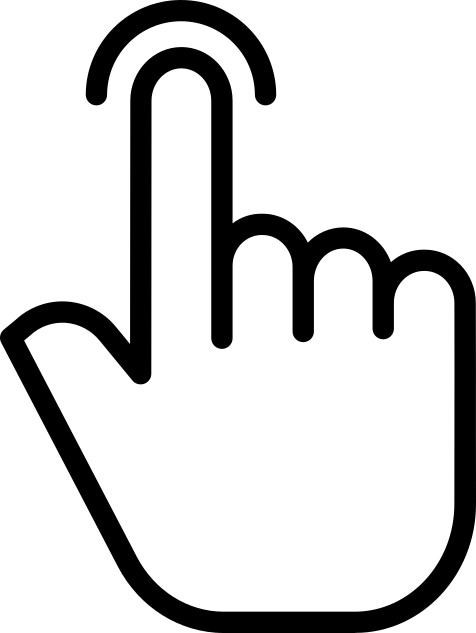
\includegraphics[width=0.05\textwidth]{static/dedo.png}} ;
    \node[const, left=of d] (nd) {\Large $s$} ;

    \edge {r} {d};
            
}
\end{figure}
\todo[inline]{¿como se interpreta la figura, que significa cada cosa?}
Siguiendo con el principio de indiferencia que usamos para definir una creencia honesta, dividimos la creencia en partes iguales por los caminos del modelo causal para definir la creencia honesta de ellos.

\begin{figure}[H]
\centering
\tikz{
\node[latent, draw=white, yshift=0.6cm] (b0) {$1$};

\node[latent,below=of b0,yshift=0.6cm, xshift=-3cm] (r1) {$r_1$};
\node[latent,below=of b0,yshift=0.6cm] (r2) {$r_2$};
\node[latent,below=of b0,yshift=0.6cm, xshift=3cm] (r3) {$r_3$};

\node[latent, below=of r1, draw=white, yshift=0.6cm] (br1) {$\frac{1}{3}$};
\node[latent, below=of r2, draw=white, yshift=0.6cm] (br2) {$\frac{1}{3}$};
\node[latent, below=of r3, draw=white, yshift=0.6cm] (br3) {$\frac{1}{3}$};
\node[latent,below=of br1,yshift=0.6cm, xshift=-0.7cm] (r1d2) {$s_2$};
\node[latent,below=of br1,yshift=0.6cm, xshift=0.7cm] (r1d3) {$s_3$};

\node[latent,below=of r1d2,yshift=0.6cm,draw=white] (br1d2) {$\frac{1}{3}\frac{1}{2}$};
\node[latent,below=of r1d3,yshift=0.6cm, draw=white] (br1d3) {$\frac{1}{3}\frac{1}{2}$};
\node[latent,below=of br2,yshift=0.6cm, xshift=-0.7cm] (r2d1) {$s_1$};
\node[latent,below=of br2,yshift=0.6cm, xshift=0.7cm] (r2d3) {$s_3$};
\node[latent,below=of br3,yshift=0.6cm, xshift=-0.7cm] (r3d1) {$s_1$};
\node[latent,below=of br3,yshift=0.6cm, xshift=0.7cm] (r3d2) {$s_2$};

\node[latent,below=of r2d1,yshift=0.6cm, draw=white] (br2d1) {$\frac{1}{3}\frac{1}{2}$};
\node[latent,below=of r2d3,yshift=0.6cm,draw=white] (br2d3) {$\frac{1}{3}\frac{1}{2}$};
\node[latent,below=of r3d1,yshift=0.6cm, draw=white] (br3d1) {$\frac{1}{3}\frac{1}{2}$};
\node[latent,below=of r3d2,yshift=0.6cm,draw=white] (br3d2) {$\frac{1}{3}\frac{1}{2}$};
\edge[-] {b0} {r1,r2,r3};
\edge[-] {r1} {br1};
\edge[-] {r2} {br2};
\edge[-] {r3} {br3};
\edge[-] {br1} {r1d2,r1d3};
\edge[-] {r1d2} {br1d2};
\edge[-] {r1d3} {br1d3};
\edge[-] {br2} {r2d1, r2d3};
\edge[-] {br3} {r3d1,r3d2};
\edge[-] {r2d1} {br2d1};
\edge[-] {r2d3} {br2d3};
\edge[-] {r3d1} {br3d1};
\edge[-] {r3d2} {br3d2};
}
\end{figure}

Primero dividimos la creencia sobre el regalo en partes iguales, y luego volvemos a dividir la creencia sobre la pista en partes iguales.
Nuestra creencia conjunta honesta a priori es,

\begin{table}[H]
\centering
 \begin{tabular}{c|c|c|c|} \setlength\tabcolsep{0.4cm} 
        & \, $r_1$ \, &  \, $r_2$ \, & \, $r_3$ \, \\ \hline 
  $s_1$ & $0$ & $1/6$ & $1/6$  \\ \hline
  $s_2$ & $1/6$ & $0$ & $1/6$  \\ \hline
  $s_3$ & $1/6$ & $1/6$ & $0$ \\ \hline 
  \end{tabular}
\end{table}
  
Es honesta porque maximiza la incertidumbre dada la información disponible hasta el momento: el modelo causal.
Y es conjunta porque es la creencia de que ocurran simultaneamente ambas variables, $\text{Creencia}(r,s)$.

% Parrafo

Habiendo definido la creencia conjunta, las creencias sobre cada una de las variables se obtiene como el total.
La creencia sobre el regalo nuevamente es 1/3,
\begin{equation}
\text{Creencia}(r_i) = \sum_j \text{Creencia}(r_i, s_j) = 1/3
\end{equation}
y sobre la pista también
\begin{equation}
\text{Creencia}(s_j) = \sum_i \text{Creencia}(r_i, s_j) = 1/3
\end{equation}

% Parrafo

Para actualizar las creencias simplemente nos quedamos con la creencia a priori que es compatible con el dato, $\text{Creencia}(r_i, s_2)$.
%
\begin{table}[H]
\centering
 \begin{tabular}{c|c|c|c|c} \setlength\tabcolsep{0.4cm} 
        & \, $r_1$ \, &  \, $r_2$ \, & \, $r_3$ \, & \\ \hline 
  $s_1$ &  &  & & \\ \hline
  $s_2$ & $1/6$ & $0$ & $1/6$ & $1/3$ \\ \hline
  $s_3$ &  &  &  & \\ \hline 
  \end{tabular}
\end{table}
%
Lo que nos permitirá cumplir el objetivo que nos habíamos propuesto, actualizar la creencia sobre el regalo luego de haber visto la pista.
Como \textbf{la creencia que sobrevive} es ahora nuestra nueva creencia total, la normalizamos (en partes iguales) para que vuelva a sumar 1
%
\begin{equation}
\text{Creencia}(r_i| s_2) = \frac{\text{Creencia}(r_i, s_2)}{\text{Creencia}(s_2)} = 1/2
\end{equation}
%
La concusión a la que llegamos coincide con la intuición de la mayoría.
\begin{figure}[H]
\centering
\tikz{ %
        
         \node[factor, minimum size=1cm] (p1) {} ;
         \node[det, minimum size=1cm, xshift=1.5cm] (p2) {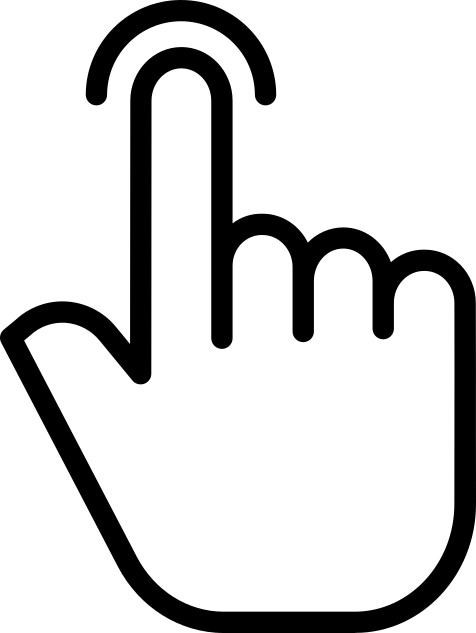
\includegraphics[width=0.03\textwidth]{static/dedo.png}} ;
         \node[factor, minimum size=1cm, xshift=3cm] (p3) {} ;

         \node[const, above=of p1, yshift=.15cm] (fp1) {$1/2$};
         \node[const, above=of p2, yshift=.15cm] (fp2) {$0$};
         \node[const, above=of p3, yshift=.15cm] (fp3) {$1/2$};
         \node[const, below=of p2, yshift=-.10cm, xshift=0.3cm] (dedo) {};
}
\end{figure}
%
Pero este resultado depende del modelo causal elegido.

\subsection{Modelos causales alternativos}

Supongamos que la pista, además de no poder coincidir con la posición del regalo, tiene prohibida una de las puertas.
Esto lo podemos representar con el siguiente modelo causal.

\begin{figure}[H]
\centering
\tikz{        
    
    \node[latent] (d) {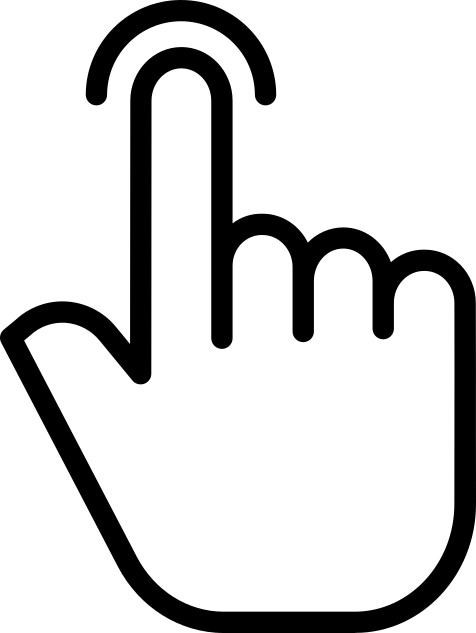
\includegraphics[width=0.05\textwidth]{static/dedo.png}} ;
    \node[const,above=of d] (nd) {\Large $s$} ;
    
    \node[latent, above=of d, xshift=-1.5cm] (r) {
\includegraphics[width=0.06\textwidth]{static/regalo.png}} ;
    \node[const,above=of r] (nr) {\Large $r$} ;
    
    \node[latent, fill=black!30, above=of d, xshift=1.5cm] (c) {
\includegraphics[width=0.06\textwidth]{static/cerradura.png}} ;
    \node[const,above=of c] (nc) {\Large $c=1$} ;
    
    \edge {r,c} {d};
}
\end{figure}

Este modelo es más conocido como el Monty Hall.
Para simplificar el problema, suponemos que la puerta 1 es la que queda cerrada, $c=1$.
Supongamos que en este contexto recibimos una pista.
%
\begin{figure}[H]
\centering
\tikz{ %
        
         \node[factor, minimum size=1cm] (p1) {
\includegraphics[width=0.025\textwidth]{static/cerradura.png}} ;
         \node[det, minimum size=1cm, xshift=1.5cm] (p2) {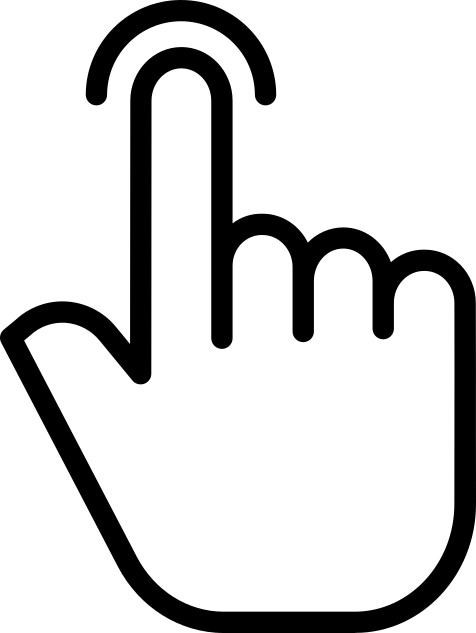
\includegraphics[width=0.03\textwidth]{static/dedo.png}} ;
         \node[factor, minimum size=1cm, xshift=3cm] (p3) {} ;
         \node[const, above=of p1, yshift=.15cm] (fp1) {$?$};
         \node[const, above=of p2, yshift=.15cm] (fp2) {$0$};
         \node[const, above=of p3, yshift=.15cm] (fp3) {$?$};
         \node[const, below=of p2, yshift=-.10cm, xshift=0.3cm] (dedo) {};
        
        } 
\end{figure}

¿Cómo hacemos para actualizar las creencias de forma honesta?
Como hicimos antes, maximizamos la incertidumbre dividiendo las creencias por los caminos del modelo causal de modo de definir la creencia conjunta honesta.

\begin{figure}[H]
\centering
\tikz{
\node[latent, draw=white, yshift=0.8cm] (b0) {$1$};
\node[latent,below=of b0,yshift=0.8cm, xshift=-2cm] (r1) {$r_1$};
\node[latent,below=of b0,yshift=0.8cm] (r2) {$r_2$};
\node[latent,below=of b0,yshift=0.8cm, xshift=2cm] (r3) {$r_3$};

\node[latent, below=of r1, draw=white, yshift=0.8cm] (br1) {$\frac{1}{3}$};
\node[latent, below=of r2, draw=white, yshift=0.8cm] (br2) {$\frac{1}{3}$};
\node[latent, below=of r3, draw=white, yshift=0.8cm] (br3) {$\frac{1}{3}$};
\node[latent,below=of br1,yshift=0.8cm] (c11) {$c_1$};
\node[latent,below=of br2,yshift=0.8cm] (c12) {$c_1$};
\node[latent,below=of br3,yshift=0.8cm] (c13) {$c_1$};

\node[latent, below=of c11, draw=white, yshift=0.8cm] (bc11) {$\frac{1}{3}$};
\node[latent, below=of c12, draw=white, yshift=0.8cm] (bc12) {$\frac{1}{3}$};
\node[latent, below=of c13, draw=white, yshift=0.8cm] (bc13) {$\frac{1}{3}$};
\node[latent,below=of bc11,yshift=0.8cm, xshift=-0.7cm] (r1d2) {$s_2$};
\node[latent,below=of bc11,yshift=0.8cm, xshift=0.7cm] (r1d3) {$s_3$};
\node[latent,below=of bc12,yshift=0.8cm] (r2d3) {$s_3$};
\node[latent,below=of bc13,yshift=0.8cm] (r3d2) {$s_2$};

\node[latent,below=of r1d2,yshift=0.8cm,draw=white] (br1d2) {$\frac{1}{3}\frac{1}{2}$};
\node[latent,below=of r1d3,yshift=0.8cm, draw=white] (br1d3) {$\frac{1}{3}\frac{1}{2}$};
\node[latent,below=of r2d3,yshift=0.8cm,draw=white] (br2d3) {$\frac{1}{3}$};
\node[latent,below=of r3d2,yshift=0.8cm,draw=white] (br3d2) {$\frac{1}{3}$};
\edge[-] {b0} {r1,r2,r3};
\edge[-] {r1} {br1};
\edge[-] {r2} {br2};
\edge[-] {r3} {br3};
\edge[-] {br1} {c11};
\edge[-] {br2} {c12};
\edge[-] {br3} {c13};
\edge[-] {c11} {bc11};
\edge[-] {c12} {bc12};
\edge[-] {c13} {bc13};
\edge[-] {bc11} {r1d2,r1d3};
\edge[-] {bc12} {r2d3};
\edge[-] {bc13} {r3d2};
\edge[-] {r1d2} {br1d2};
\edge[-] {r1d3} {br1d3};
\edge[-] {r2d3} {br2d3};
\edge[-] {r3d2} {br3d2};
}
\end{figure}

Cuando el regalo está detrás de la puerta 1, $r_1$, podemos recibir una pista tanto en la puerta 2, $s_2$, como en la puerta 3, $s_3$.
Si el regalo está en la puerta 2, $r_2$, la pista sólo puede señalar la puerta 3, $s_3$.
Así definimos la siguiente creencia honesta conjunta (y sus marginales).

\begin{table}[H]
\centering
 \begin{tabular}{c|c|c|c||c} \setlength\tabcolsep{0.4cm} 
        & \, $r_1$ \, &  \, $r_2$ \, & \, $r_3$ \, & \\ \hline 
  $s_2$ & $1/6$ & $0$ & $1/3$ & $1/2$ \\ \hline
  $s_3$ & $1/6$ & $1/3$ & $0$ & $1/2$ \\ \hline \hline 
  & $1/3$& $1/3$ & $1/3$ & $1$
  \end{tabular}
 \end{table}
 
Para actualizar nuestra creencia, nuevamente nos quedamos con la creencia a priori que es compatible con los datos.

\begin{table}[H]
\centering
 \begin{tabular}{c|c|c|c||c} \setlength\tabcolsep{0.4cm} 
        & \, $r_1$ \, &  \, $r_2$ \, & \, $r_3$ \, &  \\ \hline 
  $s_2$ & $1/6$ & $0$ & $1/3$ & $1/2$ \\ \hline
  \end{tabular}
\end{table}

Que normalizado en partes iguales para que sume 1 queda como

\begin{figure}[H]
\centering
\tikz{ %
        
         \node[factor, minimum size=1cm] (p1) {
\includegraphics[width=0.025\textwidth]{static/cerradura.png}} ;
         \node[det, minimum size=1cm, xshift=1.5cm] (p2) {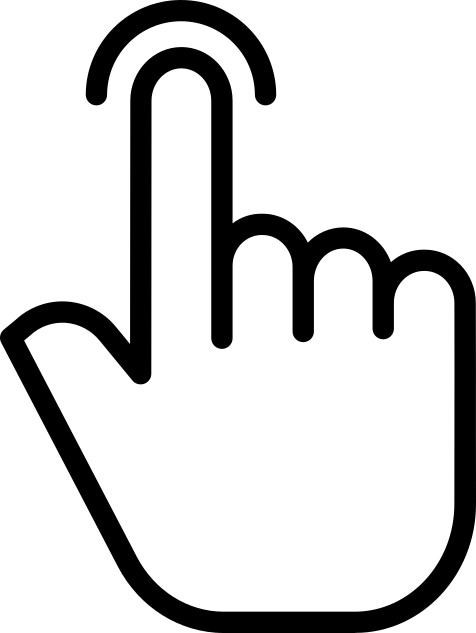
\includegraphics[width=0.03\textwidth]{static/dedo.png}} ;
         \node[factor, minimum size=1cm, xshift=3cm] (p3) {} ;
         
         \node[const, above=of p1, yshift=.15cm] (fp1) {$1/3$};
         \node[const, above=of p2, yshift=.15cm] (fp2) {$0$};
         \node[const, above=of p3, yshift=.15cm] (fp3) {$2/3$};
         \node[const, below=of p2, yshift=-.10cm, xshift=0.3cm] (dedo) {};
        } 
\end{figure}
  
Esta respuesta es diferente a la que obtuvimos con el primer modelo causal.
Sin embargo, ambas comparten la propiedad de ser la distribución de creencias que maximiza la incertidumbre dada la evidencia formal (modelo causal) y empírica (datos), lo que hace que sean proposiciones sobre las que podemos acordar tanto intercultural como intersubjetivamente.

\section{Reglas de la probabilidad}

Las reglas de la probabilidad han sido derivadas formalmente a partir de una gran cantidad de sistemas axiomáticos conceptualmente distintos e independientes entre si, lo cual es uno de los punto fuertes a su favor.
Pero quizás más importante es que ellas garantizan maximizar la incertidumbre dada la información empírica (datos) y formal (modelos causales).

% Parrafo

La teoría de la probabilidad tiene sólo dos reglas, conocidas como la regla de la suma y la regla del producto.
La primera regla computa la creencia de una variable simplemente como el total que ya le fue asignado en la creencia conjunta.
\begin{equation}
P(r_i) = \sum_j P(r_i, s_j)
\end{equation}
La segunda regla simplemente se queda con nueva creencia total a la creencia a priori que es compatible con el dato.
Expresada como producto
\begin{equation}
P(s_j)P(r_i|s_j) = P(r_i, s_j)
\end{equation}

Toda la teoría de la probabilidad se reduce a estas dos reglas.

\subsection{Teorema de Bayes}

El teorema de Bayes no es más que un corolario de las reglas de las probabilidad.

\begin{equation}
\begin{split}
P(r_i|s_2) = \frac{P(r_i, s_2)}{P(s_2)} = \frac{P(s_2|r_i)P(r_i)}{P(s_2)} 
\end{split}
\end{equation}

En términos más generales, $r_i$ representa las hipótesis y $s_2$ reṕresenta el dato.

\begin{equation*}
\underbrace{P(\text{Hip\'otesis }|\text{ Datos})}_{\text{\scriptsize Posteriori}} = \frac{\overbrace{P(\text{Datos }|\text{ Hip\'otesis})}^{\text{\scriptsize Verosimilitud}} \overbrace{P(\text{Hip\'otesis})}^{\text{\scriptsize Priori}} }{\underbrace{P(\text{Datos})}_{\text{\scriptsize Evidencia}}}
\end{equation*}

Es importante notar que todas estas probabilidades en realidad dependen de un cierto modelo causal, por lo correcto sería incluirlo explícitamente en el condicional.


\begin{equation*}
\underbrace{P(\text{Hip\'otesis }|\text{ Datos, Modelo})}_{\text{\scriptsize Posteriori}} = \frac{\overbrace{P(\text{Datos }|\text{ Hip\'otesis, Modelo})}^{\text{\scriptsize Verosimilitud}} \overbrace{P(\text{Hip\'otesis }|\text{ Modelo})}^{\text{\scriptsize Priori}} }{\underbrace{P(\text{Datos }|\text{ Modelo})}_{\text{\scriptsize Evidencia}}}
\end{equation*}

\subsection{Verosimilitud}

La verosimilitud es la predicción de los datos dada las hipótesis.
Veamos cuál es la verosimilitud, $P(s2|r_i)$, en el modelo de Monty Hall.

\begin{figure}[H]
\centering
\tikz{
\phantom{\node[latent, draw=white, yshift=0.8cm] (b0) {$1$};}
\node[latent,below=of b0,yshift=0.8cm, xshift=-3cm] (r1) {$r_1$};
\node[latent,below=of b0,yshift=0.8cm] (r2) {$r_2$};
\node[latent,below=of b0,yshift=0.8cm, xshift=3cm] (r3) {$r_3$};

\node[latent, below=of r1, draw=white, yshift=0.8cm] (br1) {$1$};
\node[latent, below=of r2, draw=white, yshift=0.8cm] (br2) {$1$};
\node[latent, below=of r3, draw=white, yshift=0.8cm] (br3) {$1$};
\node[latent,below=of br1,yshift=0.8cm] (c11) {$c_1$};
\node[latent,below=of br2,yshift=0.8cm] (c12) {$c_1$};
\node[latent,below=of br3,yshift=0.8cm] (c13) {$c_1$};

\node[latent, below=of c11, draw=white, yshift=0.8cm] (bc11) {$1$};
\node[latent, below=of c12, draw=white, yshift=0.8cm] (bc12) {$1$};
\node[latent, below=of c13, draw=white, yshift=0.8cm] (bc13) {$1$};
\node[latent,below=of bc11,yshift=0.8cm, xshift=-0.7cm] (r1d2) {$s_2$};
\node[latent,below=of bc11,yshift=0.8cm, xshift=0.7cm] (r1d3) {$s_3$};
\node[latent,below=of bc12,yshift=0.8cm] (r2d3) {$s_3$};
\node[latent,below=of bc13,yshift=0.8cm] (r3d2) {$s_2$};

\node[latent,below=of r1d2,yshift=0.8cm,draw=white] (br1d2) {$\frac{1}{2}$};
\node[latent,below=of r1d3,yshift=0.8cm, draw=white] (br1d3) {$\frac{1}{2}$};
\node[latent,below=of r2d3,yshift=0.8cm,draw=white] (br2d3) {$1$};
\node[latent,below=of r3d2,yshift=0.8cm,draw=white] (br3d2) {$1$};
\phantom{\edge[-] {b0} {r1,r2,r3};}
\edge[-] {r1} {br1};
\edge[-] {r2} {br2};
\edge[-] {r3} {br3};
\edge[-] {br1} {c11};
\edge[-] {br2} {c12};
\edge[-] {br3} {c13};
\edge[-] {c11} {bc11};
\edge[-] {c12} {bc12};
\edge[-] {c13} {bc13};
\edge[-] {bc11} {r1d2,r1d3};
\edge[-] {bc12} {r2d3};
\edge[-] {bc13} {r3d2};
\edge[-] {r1d2} {br1d2};
\edge[-] {r1d3} {br1d3};
\edge[-] {r2d3} {br2d3};
\edge[-] {r3d2} {br3d2};
}
\end{figure}

\begin{table}[H]
\centering
 $P(s_2|r_i)$   
 
 \begin{tabular}{c|c|c|c} \setlength\tabcolsep{0.4cm} 
          & \, $r_1$ \, &  \, $r_2$ \, & \, $r_3$ \, \\ \hline 
   $s_2$ & $1/2$ & $0$ & $1$  \\ \hline
\end{tabular}
\end{table}

\subsection{Posterior}

\subsection{Evidencia}




\section{Selección de modelos}

\chapter{TrueSkill Through Time}

\chapter{Las implementaciones en Julia, Python y R}

\chapter{Efecto de los equipos sobre el aprendizaje (faithfull-sinergia)}

\chapter{Efecto de la topología sobre el aprendizaje.}

\chapter{Sistema de estimación para el juego Go (AAGo).}


\end{document}
